\documentclass[compress,hyperref={linkcolor=blue,pdftex,unicode}]{beamer}
\usepackage[utf8]{inputenc}
\usepackage[english,russian]{babel}

\ifpdf
        \usepackage{cmap} % чтобы работал поиск по PDF
\fi


\usepackage{eurosym}
\usepackage{xspace}
\usetheme{PaloAlto}
\usecolortheme{seahorse}

\usefonttheme[onlysmall]{structurebold}
\setbeamerfont{title}{shape=\itshape,family=\rmfamily}
\setbeamercolor{title}{fg=red!80!black,bg=red!20!white}
\setbeamercolor{alerted text}{fg=blue}
\setbeamercovered{highly dynamic}

\newcommand{\myeuro}{\textcolor{blue}{\it\euro}\xspace}
\newcommand{\myhref}[2]{\textcolor{blue}{\href{#1}{#2}}}


\date{March 11, 2011}
\author[]{\myhref{mailto:vitaly.repin@nokia.com}{В.А. Репин}\\ MeeGo Computers, Nokia}
\title[\tiny QMF, E-Mail в MeeGo]{Qt Messaging Framework и подсистема электронной почты в MeeGo}
\institute[\tiny MeeGo]{MeeGo}

\logo{\resizebox{!}{0.4cm}{
\includegraphics{nokia}}}

\begin{document}
\large

\begin{frame}
\titlepage
\end{frame}

\begin{frame}
\frametitle{E-mail в Linux-платформах, поддерживаемых Nokia. Краткий исторический экскурс.}
\begin{description}
\item[2005 г.] Интернет-таблетка N770. Там \textbf{уже} был почтовый клиент :-)
\pause
\item[2007 г.] Интернет-таблетка N800. Modest. libcamel/tinymail
\pause
\item[2007 г.] Интернет-таблетка N810. Modest. libcamel/tinymail
\pause
\item[2009 г.] Первый Linux-телефон Nokia, N900. Modest. libcamel/tinymail. Первое появление QMF (в несколько урезанном виде)
на платформе
\pause
\item[2010 г.] Рождение MeeGo. QMF - в MeeGo. Qt.
\end{description}
\end{frame}

\begin{frame}
\frametitle{Архитектура Qt Messaging Framework}
\centerline{\resizebox{\textwidth}{!}{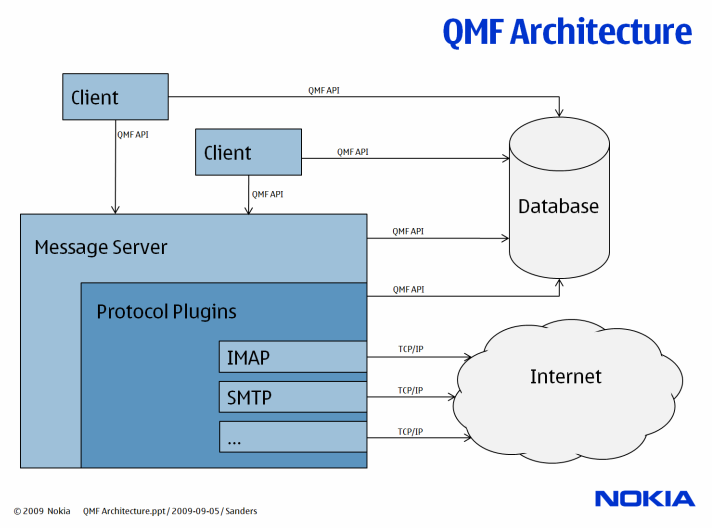
\includegraphics{qmf-architecture}}}
\end{frame}

\begin{frame}
\frametitle{QMF. Коротко о главном.}
\begin{itemize}
\item C++/Qt. Опасности - граната и обезьяна. Не наш случай.
\pause
\item Кросс-платформенность (Linux, S60, Win, Mac)
\pause
\item Расширяемость протокольного стека. В базовую поставку входят IMAP-4 (Lemonade), POP-3, SMTP
\pause
\item Адаптируемость к новым платформам (PIMPL), четкое отделение UI и backend
\pause
\item Открытость исходного кода
\pause
\item Модели данных Qt: \texttt{QMailMessageThreadedModel, QMailAccountListModel...}
\pause
\item Service actions:  \texttt{QMailRetrievalAction, QMailSearchAction, QMailTransmitAction...}
\pause
\item Протокольные плагины: \texttt{QMailMessageSink, QMailMessageSource}
\end{itemize}
\end{frame}

\begin{frame}
\frametitle{QMF в N900}
\begin{itemize}
\item Хранилище E-Mail базы MfE (ActiveSync)
\pause
\item Интеграция с modest через modest plugin и libcamel provider. Использование Qt из кода libcamel provider.
\pause
\item Увеличение скорости разработки, повышение качества ПО и обкатка новой технологии не всегда конфликтуют!
\pause
\item as-daemon: \textbf{0 crashes} в sales release.
\pause
\item Небольшое лирическое отступление - протокольные провайдеры в libcamel и плагины к Modest.
\end{itemize}
\end{frame}

\begin{frame}
\frametitle{QMF-ресурсы}
\begin{itemize}
\item Gitorius: \myhref{http://qt.gitorious.org/qt-labs/messagingframework}{http://qt.gitorious.org/qt-labs/messagingframework}
\pause
\item Список рассылки для разработчиков (англоязычный): \myhref{mailto:qt-qmf@qt.nokia.com}{qt-qmf@qt.nokia.com}
\pause
\item Список рассылки для русскоязычных пользователей: \myhref{mailto:qmf-users-rus@freelists.org}{qmf-users-rus@freelists.org}
\end{itemize}
\end{frame}

\begin{frame}
\frametitle{Спасибо за внимание! Вопросы? Предложения?}
\centerline{\resizebox{0.8\textwidth}{!}{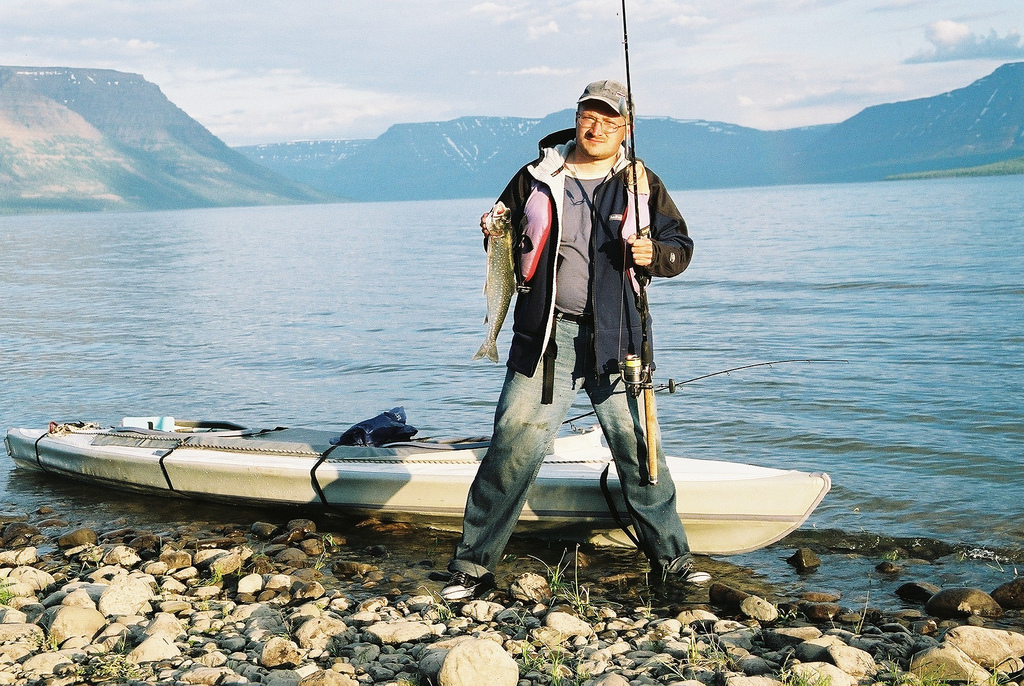
\includegraphics{qs}}}

\begin{center}
\huge\bf \myhref{mailto:vitaly.repin@nokia.com}{vitaly.repin@nokia.com}
\end{center}
\end{frame}

\end{document}
